
\section{Results}
\label{sec:results}

\begin{figure}[htb]

  \centering  % centers the image in the column

  % replace the second argument below with your filename. I like to
  % place all my figures in a sub-directory to keep things organized
  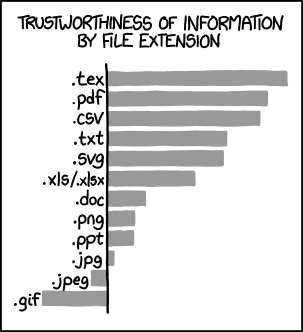
\includegraphics[width=0.47\textwidth]{figs/file_extensions.png}

  % *Every* figure should have a descriptive caption.
  \caption{On the trustworthiness of \LaTeX. Image courtesy of \texttt{xkcd}.}
  \label{fig:tex}

\end{figure}

\subsection{Creating Tables}
\label{subsec:tables}

\begin{figure}[htb]
  \centering % centers the entire table

  \begin{tabular}{c|c|c|}

     & Elastic or Not & % Error \\ % separate column contents using the &
    \hline % line after the column headers
    SGD & with &  \\
    SGD & without &  \\
    SVM & with &  \\
    SVM & without &  \\
    MLP Identity & with &  \\
    MLP Identity & without &  \\
    MLP Rectified & with &  \\
    MLP Rectified & without &  \\
    \hline \hline
  \end{tabular}

  \caption{An example table.}
  \label{tab:example}

\end{figure}
